\section{基于Armjio步长的梯度下降法}
\subsection{问题}
利用基于Armjio步长梯度下降法求解以下问题:
\begin{equation}\label{eq:Armjio}
    f(\boldsymbol{x}) = 100\times (x_2-x_1^2)^2+(1-x_1)^2
\end{equation}
\subsection{方法}
最优步长的缺陷:
\begin{itemize}
    \item 最优步长的初衷是在每一迭代步使目标函数下降量达到最大.但计算量太大,而且不好求. 
    \item 最优化问题关注全局最优值点。集中于某个方向上的线搜索似乎没有必要。
\end{itemize}

设$\boldsymbol{d}_k$为$\boldsymbol{x}_k$的下降方向,即$\boldsymbol{d}_{k}^{\mathrm{T}}\boldsymbol{g}_k<0$,对$\sigma\in\left( 0,1 \right)$,只要$\alpha>0$充分小,有
\[
    f(\boldsymbol{x}_k+\alpha\boldsymbol{d}_k) = f(\boldsymbol{x}_k)+\alpha \boldsymbol{g}_{k}\boldsymbol{d}_k+o(\alpha)<0
\]

步长选取:先取一个较大的步长, 看目标函数是否有满意的下降量。否则依次按比例压缩,直至满足要求。又称进退试探法。
\begin{definition}[Armijo步长规则]
    取常数$\beta>0,\sigma,\gamma\in(0,1)$。步长$\alpha_k = \beta \gamma^{m_k}$,其中$m_k$为$0,1,\cdots$中满足下式的最小值
    \[
        f(\boldsymbol{x}_k+\beta\gamma^{m_{k}}\boldsymbol{d}_k) \leqslant f_k+\sigma\beta\gamma^{m_{k}}\boldsymbol{g}_k^{\mathrm{T}}\boldsymbol{d}_k
    \]

    如$\alpha_k<\beta$,则
    \[
        \begin{array}{c}
            f(\boldsymbol{x}_k+\beta\gamma^{\colorbox{red!30}{$m_k$}}\boldsymbol{d}_k)\leqslant f(\boldsymbol{x}_k)+\sigma\beta\gamma^{m_k}\boldsymbol{g}_k^{\mathrm{T}}\boldsymbol{d}_k\\
            f(\boldsymbol{x}_k+\beta\gamma^{\colorbox{red!30}{$m_k-1$}}\boldsymbol{d}_k)> f(\boldsymbol{x}_k)+\sigma\beta\gamma^{m_k-1}\boldsymbol{g}_k^{\mathrm{T}}\boldsymbol{d}_k
        \end{array}
    \]
\end{definition}

将Armijo步长规则写为伪代码见算法~\ref{alg:Armijo}。

\begin{algorithm}[H]
    \SetAlgoLined
    \caption{Armijo步长规则}
    \label{alg:Armijo}
    \KwIn{当前迭代点$\boldsymbol{x}$,下降方向$\boldsymbol{d}$,优化函数$f$,梯度函数$\nabla f$}
    \KwOut{Armijo步长$\alpha$}
    $m_{k} = 0,\beta>0,\sigma,\gamma\in(0,1)$\\
    \While{$ f(\boldsymbol{x}+\beta\gamma^{m_{k}}\boldsymbol{d}) > f(\boldsymbol{x})+\sigma\beta\gamma^{m_{k}}\nabla f(\boldsymbol{x})^{\mathrm{T}}\boldsymbol{d} $}{
        \eIf{$ f(\boldsymbol{x}+\beta\gamma^{m_{k}}\boldsymbol{d}) \leqslant f(\boldsymbol{x})+\sigma\beta\gamma^{m_{k}}\nabla f(\boldsymbol{x})^{\mathrm{T}}\boldsymbol{d} $}{
            \textbf{break}
        }{
            $m_k \gets m_{k} + 1$
        }
    }
    $\alpha \gets \beta\gamma^{m_{k}}$\\
    \Return{$\alpha$}
\end{algorithm}
\subsection{结果}
运行``main.m''得到迭代序列如图~\ref{fig:Armijo-matlab}。
\begin{figure}[htbp]
    \centering
    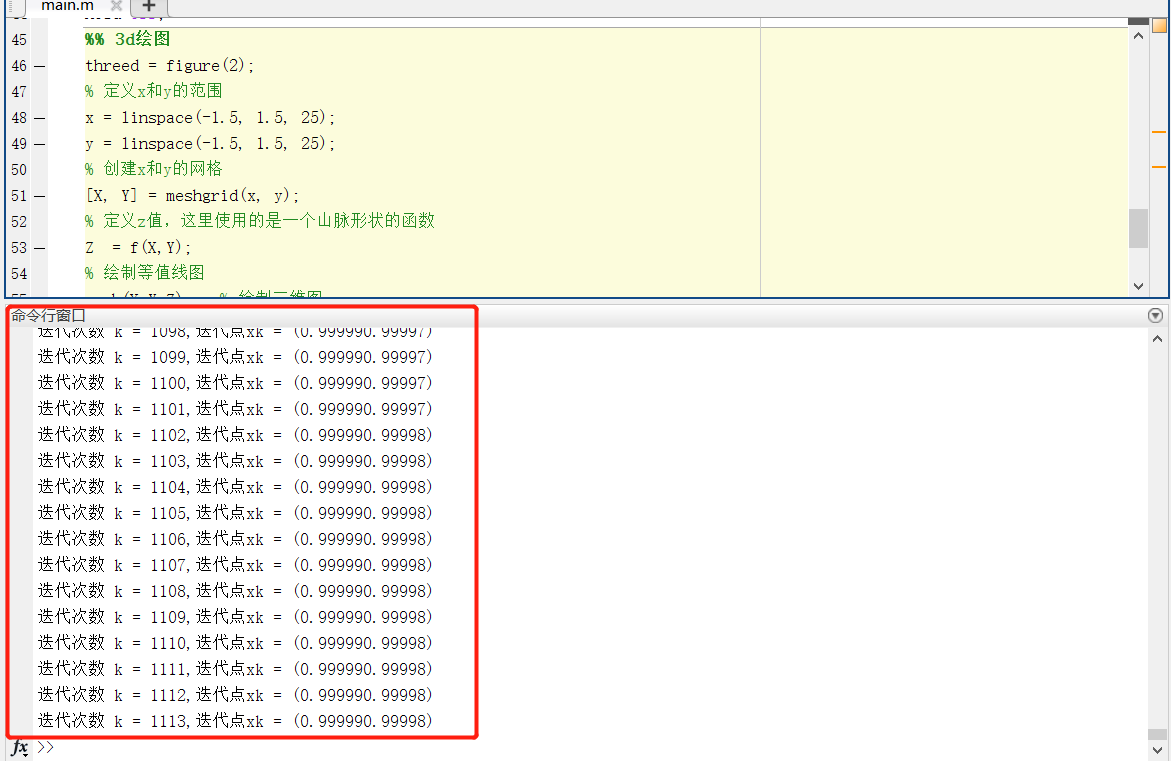
\includegraphics[width = .8\textwidth]{image/armijo.png}
    \caption{运行`main.m'得到迭代序列}
    \label{fig:Armijo-matlab}
\end{figure}

算法求解问题~(\ref{eq:Armjio})得到的数值最优解$\boldsymbol{x}^*$
\[
    \boldsymbol{x}^* = \left( 0.999990,0.99998 \right)^{\mathrm{T}}
\]

算法迭代过程如图~\ref{fig:Armijo}。
\begin{figure}[htbp]
    \centering%
    \subfloat[基于Armjio步长的梯度下降法2d迭代]{%
        \label{fig:Armijo-2d}
        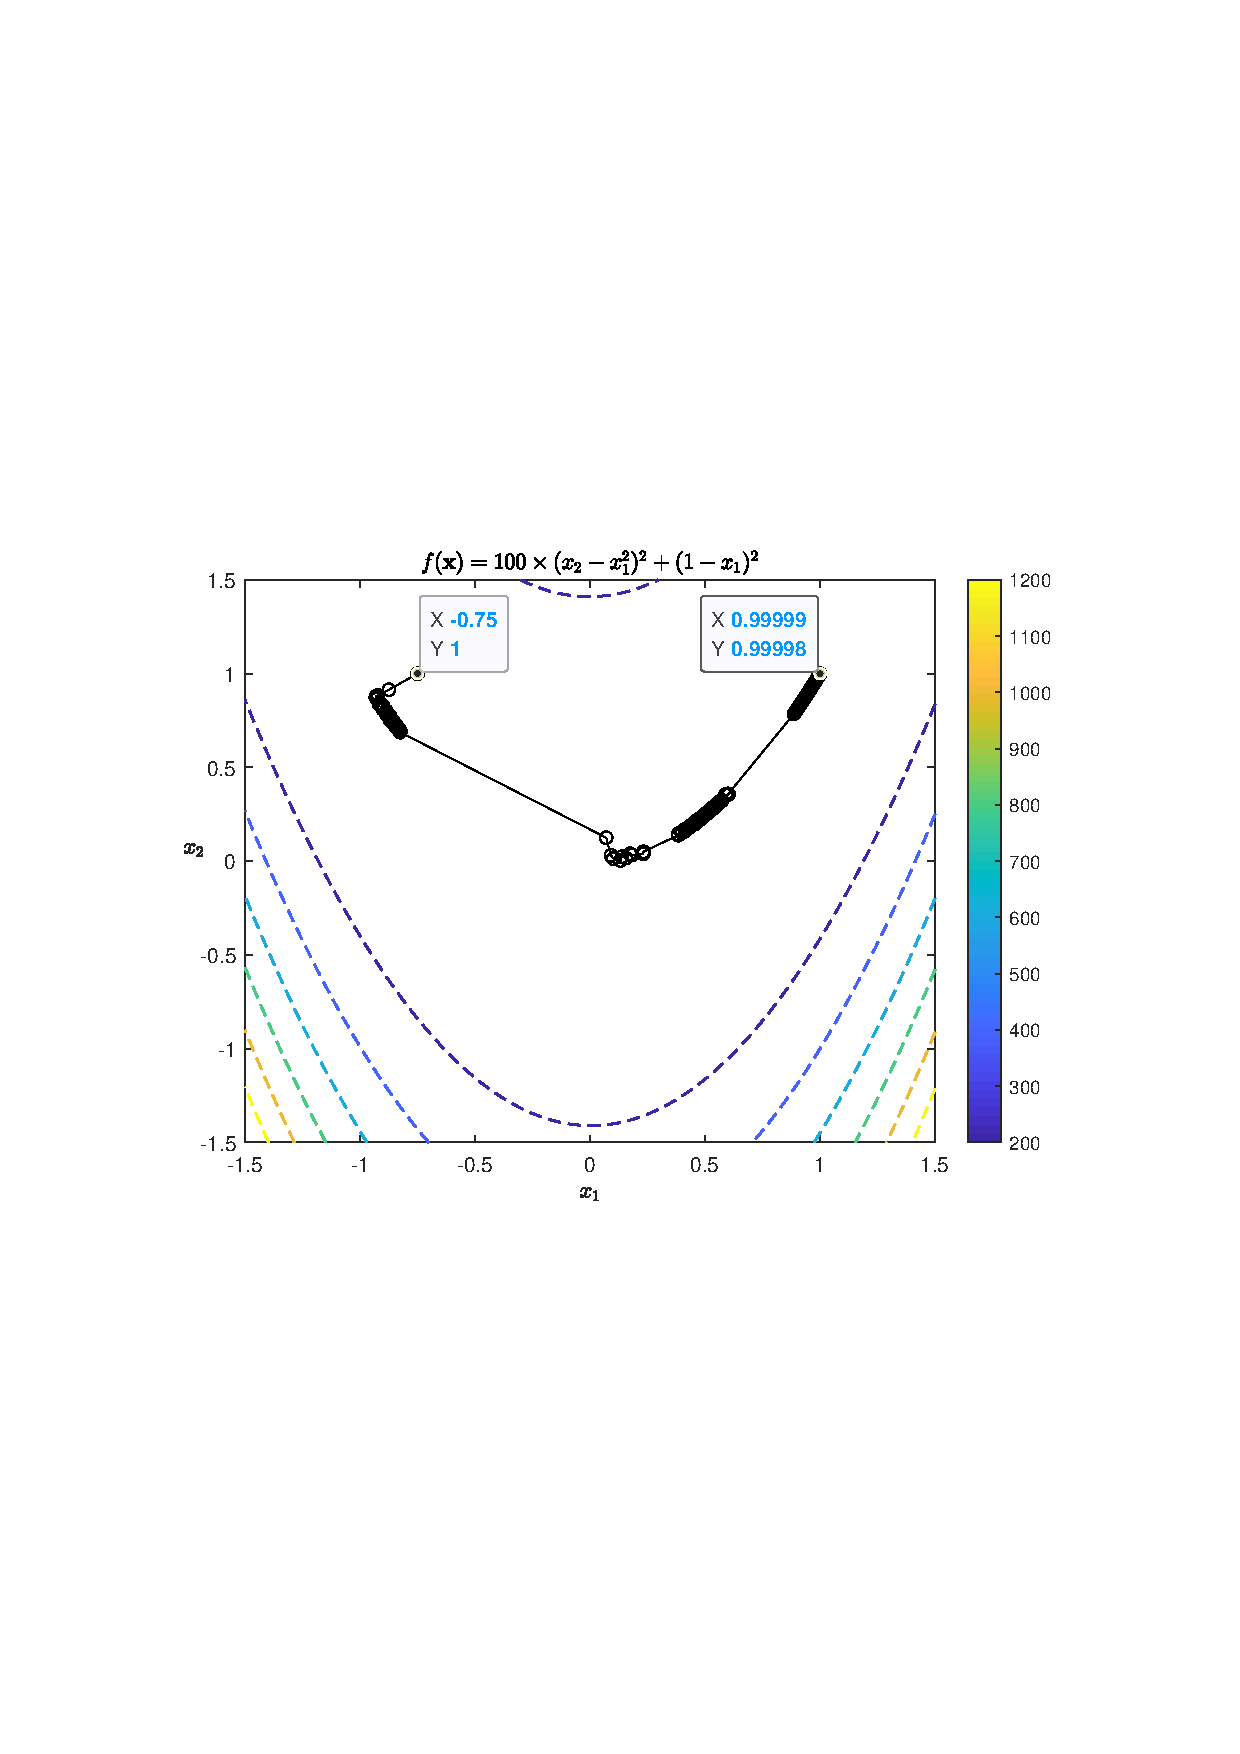
\includegraphics[width = .45\textwidth]{image/armijo.pdf}}\hspace{.5em}%
    \subfloat[基于Armjio步长的梯度下降法3d迭代]{%
      \label{fig:Armijo-3d}
      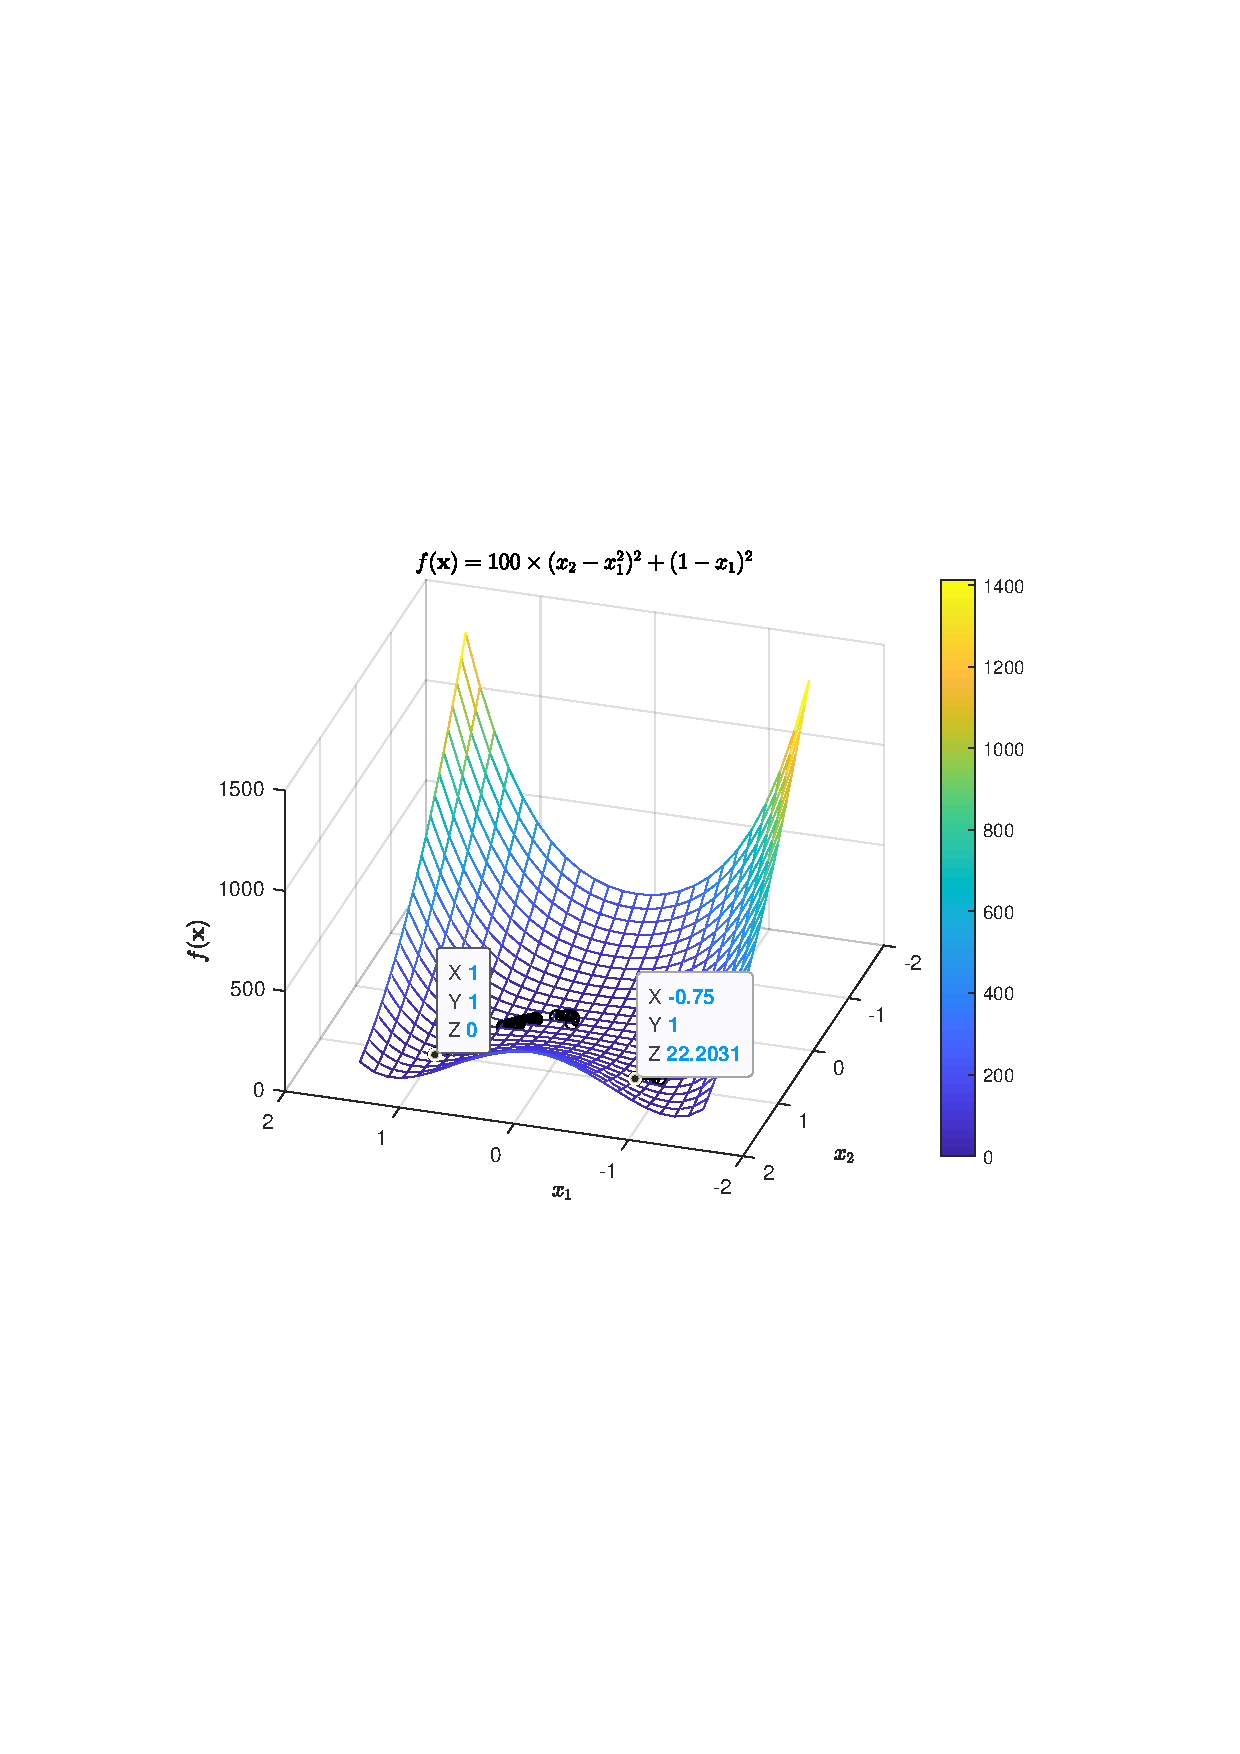
\includegraphics[width = .45\textwidth]{image/armijo-3d.pdf}}
    \caption{基于Armjio步长的梯度下降法}
    \label{fig:Armijo}
\end{figure}
\subsection{代码}
Armijo步长和主函数见代码~\ref{code:Armijo}和~\ref{code:Armijo-main}。
\lstinputlisting[
    language    =   matlab,
    style       =   elegantcode,
    caption     =   {Armjio步长代码},
    label       =   {code:Armijo}
]{code/armijo.m}
\lstinputlisting[
    language    =   matlab,
    style       =   elegantcode,
    caption     =   {主函数代码},
    label       =   {code:Armijo-main}
]{code/main.m}